\documentclass{beamer}
\usepackage[spanish]{babel}
\usepackage[utf8]{inputenc}
\usepackage{multicol}
\useoutertheme{tree}
\usetheme{Berlin}
\usepackage{framed, color}
\definecolor{shadecolor}{rgb}{0.6078,0.651,0.651}
\date{1 de Julio de 2016}
%\usecolortheme{lily}
\useoutertheme{shadow}
\useinnertheme{rectangles}
\title{\textbf{Shiny de RStudio}}
\subtitle{\textit{Framework de R para aplicaciones Web}}
\author[Briggette Román]{\textbf{Briggette Olenka Román Huaytalla}\\Facultad de Ciencias\\Grupo Estudiantil ACECOM\\Universidad Nacional de Ingeniería}
 \AtBeginSection{ 
 	\begin{frame} 
 		\frametitle{Índice}
 		\tableofcontents[currentsection]
 	\end{frame}
 }
 
 \AtBeginSubsection{ 
 	\begin{frame}
 		\frametitle{Índice}
 		\tableofcontents[currentsection,currentsubsection]
 	\end{frame}
 }
\begin{document}
	\maketitle
	
\begin{frame}
	\frametitle{Índice}
	\begin{multicols}{2}
		\tableofcontents
	\end{multicols} 
\end{frame}

\section{Introducción}
\begin{frame}
    \frametitle{Introducción}
    Shiny es un framework de RStudio con el cual nos permite hacer aplicaciones web, pudiendo así trabajar de manera dinámica con los datos para un presentación o para que el usuario final le facilite la manera de ingresar o obtener resultados de la bases de datos procesadas.
    \begin{figure}[h!]
    	
\includegraphics[scale=0.1]{rstudio}
    \end{figure}
\end{frame}
\section{¿Cómo empezar?}
\begin{frame}
	\frametitle{¿Cómo empezar?}
	Primero es instalar el paquete \emph{shiny}:
	
	\begin{block}{}
		$>>$ install.package("shiny")
	\end{block}
	
	\textbf{Tener cuidado} que repositorio se elija para descargar ya que algunos no funcionan correctamente en este caso se usó el \textit{repositorio de España Madrid}.\\\
	
	\textit{** Esto es en caso de que se este trabajando desde terminal}

\end{frame}
\begin{frame}[fragile]
	\frametitle{¿Cómo empezar? - Parte 2}
	\begin{multicols}{2}
		Ahora trabajando desde el IDE de Rstudio primero es instalar el paquete \emph{shiny}:
		
		\begin{verbatim}
		> install.package("shiny")
		\end{verbatim}
		Que al ejecutar nos mostrara en la consola del editor como se muestra en la imagen.
		\begin{figure}[h!]
			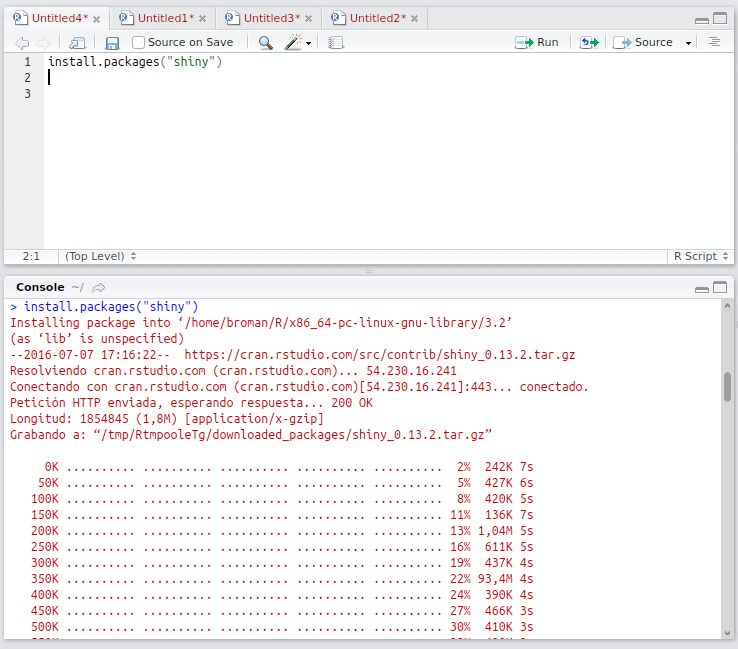
\includegraphics[scale=0.2]{instalacion}
		\end{figure}
	\end{multicols} 
	
\end{frame}
\section{IDE}
\subsection{RStudio}
\begin{frame}
	\frametitle{¿Como ejecutar? }
	\begin{multicols}{2}
		La manera en como trabaja shiny nos permitirá ver ejecución de nuestro trabajo en distintas maneras. Teniendo el siguiente panel en nuestro IDE.
		\begin{figure}[h!]
			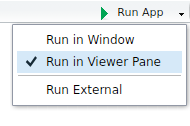
\includegraphics[scale=0.5]{run}
		\end{figure}
		
		\begin{itemize}
			\item \textbf{Run in Window}, se ejucatara dentro del IDE en la ventana de trabajo.
			\item \textbf{Run in Viewer Pane}, se abrirá un panel externo para visualizar nuestra ejecución.
			\item \textbf{Run in external},  se ejecutara nuestro programa en un navegador web. En este caso \textit{Chrome}
		\end{itemize}
	\end{multicols}
	\textit{** Porque las diferencias, debido a que así uno pude visualizar como quedara para el usuario.}
\end{frame}
\subsection{Trabajando con Shiny}
\begin{frame}[fragile]
	\frametitle{Empezando: }
	En todos nuestros programas que realizaremos usando el framework de shiny comenzaremos llamando a la librería de \emph{shiny}
	
	\begin{verbatim}
		> library(shiny)
	\end{verbatim}
	
	
	%	\begin{figure}[h!]
	%		
\includegraphics[scale=0.1]{rstudio}
	%	\end{figure}
\end{frame}
\begin{frame}[fragile]
	\frametitle{Shiny}
	Habiendo encabezado el programa con la librería \textit{\textbf{shiny}} se empieza a armar el código con dos secciones una que es para la edición frontal(La parte en que se muestra en ejecución la interfaz de Usuario o UI) que seria el \textbf{fluidPage}  y la parte que trabaja internamente que seria el \textbf{server} 
	
	\begin{verbatim}
		library(shiny)
		ui <- fluidPage( 
		    ...
		)
		
		server <- function(input, output){
		    ...	
		}
		
		shinyApp(ui = ui, server = server)
	\end{verbatim}

\end{frame}

\begin{frame}[fragile]
	
	\frametitle{Ejemplo}
	\begin{verbatim}
		library(shiny)
		ui <- fluidPage(
		    sliderInput(inputId = "num",
		    label = " Elige un número",
		    value = 50, min = 1 , max=100),
		    plotOutput("hist")
		)
		server <- function(input, output){
		    output \textdollar hist<-renderPlot({
		    title <-"Histograma de datos"
		    hist(rnorm(input\textdollar num))
		    main = title	
		    })
		}
		shinyApp(ui =ui,server = server)
	\end{verbatim}
	
	
	%	\begin{figure}[h!]
	%		
\includegraphics[scale=0.1]{rstudio}
	%	\end{figure}
\end{frame}
\begin{frame}
	\frametitle{Ejemplo: Ejecución }
	En el cual nos aparecerá algo como esto:
	
		\begin{figure}[h!]
			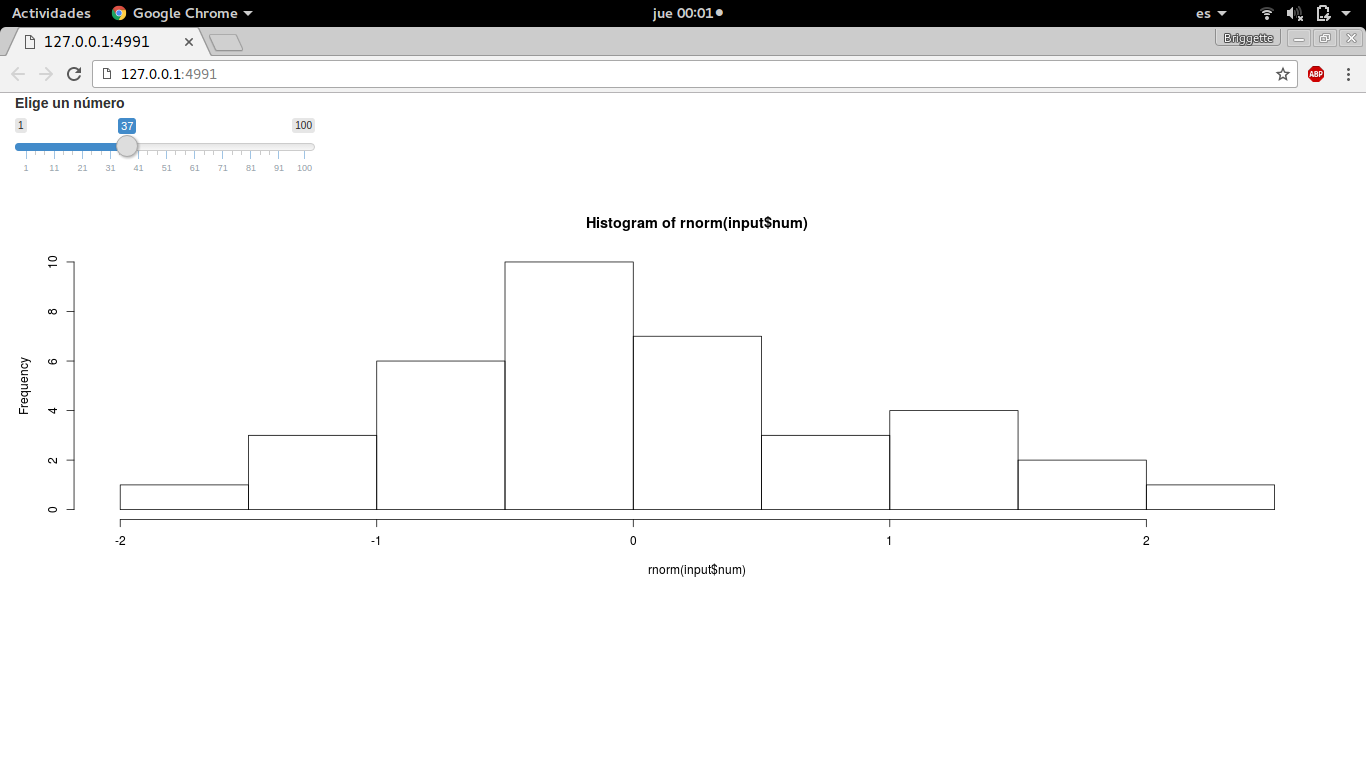
\includegraphics[scale=0.2]{example1}
		\end{figure}
\end{frame}
\subsection{Trabajando con Shiny - División del trabajo}
\begin{frame}
	\frametitle{¿Como trabaja shiny realmente? }
	Shiny trabaja  dividiendo su trabajo en dos secciones en las cuales una es la parte de \textbf{UI}(\textit{User interface}) y la otra es la de \textbf{server}(que es donde procesa la data obtenida o almacenada).
	
	\begin{figure}[h!]
		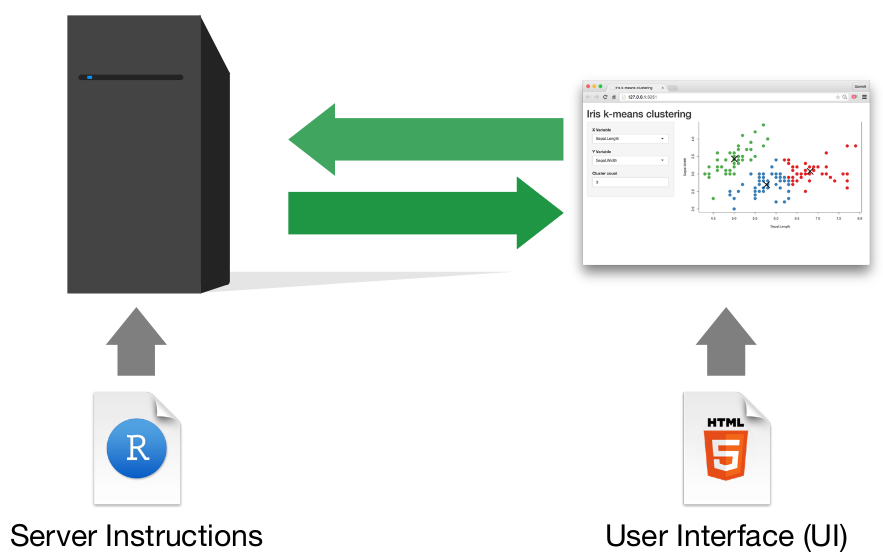
\includegraphics[scale=0.2]{arquitectura}
	\end{figure}
\end{frame}
\begin{frame}[fragile]
	\frametitle{División del programa: Estructura}
	Ahora se trabajara con archivos independientes donde uno trabajara la parte de \textit{FrontEnd} osea la \textbf{UI} y la parte de \textit{BackEnd} que seria la parte de \textbf{Server}. Teniendo la estructura siguiente
	
\textbf{	Primer Archivo:}\textit{ ui.R}
	\begin{verbatim}
		#ui.R
		library(shiny)
		   shinyUI( fluidPage( ...
		   ))
	\end{verbatim}
	
\textbf{	Segundo archivo:}\textit{ server.R}
	\begin{verbatim}
		#server.R
		library(shiny)
		    shinyServer(
		        function(input, output){...
		    })
	\end{verbatim}
		
\end{frame}

\begin{frame}[fragile]
\frametitle{Ejemplo: \textbf{ui.R}}
\begin{verbatim}
library(shiny)
shinyUI(
    fluidPage(
        titlePanel("Shiny App"),
        sidebarLayout(
            sidebarPanel(
                sliderInput(inputId = "num",
                    label = "Elige un número",
                    value = 50, min = 1, max = 100)
            ),
            mainPanel(
                plotOutput("distPlot")
            )
        )
    )
)
\end{verbatim}
\end{frame}
\begin{frame}[fragile]
	\frametitle{Ejemplo: \textbf{server.R}}
	\begin{verbatim}
	library(shiny)
	shinyServer(
	    function(input, output){
	        data <-reactive({
	            rnorm(input$num)
	        })
	        output$distPlot <- renderPlot({
	            hist(rnorm(input$num))
	        })
	    }
	
	)
	\end{verbatim}
\end{frame}

\begin{frame}[fragile]
	\frametitle{Formas de ejecución:}
	Ahora si bien puedes ejecutar tu programa en ese momento cuando estas editandolo, que pasa ahora que desees ejecutarlo externamente o llamarlo desde otro programa.
	Para ello debes haber guardado tus archivos \textit{ui.R }y \textit{server.R} en una carpeta o directorio,que en este caso estan en \textit{Escritorio/primerAppShiny} , para poder correrlo de la siguiente manera:
	\begin{verbatim}
	> library(shiny)
	> runApp('ubicacion/del/directorio/de/tu/app')
	\end{verbatim}
	
	\textbf{Ejemplo: }
	\begin{verbatim}
	> library(shiny)
	> runApp('Escritorio/primerAppShiny')
	\end{verbatim}
\end{frame}
\end{document}